\documentclass[runningheads]{llncs}

\usepackage{graphicx}
\usepackage[english]{babel}
\usepackage{amsmath}
\usepackage{amsfonts}
\usepackage{textcomp}
\usepackage{multirow}
\usepackage{subfigure}

\graphicspath{{tavaeva/}}

\begin{document}

\title{A Cost Minimizing at Laser Cutting of Sheet Parts on CNC Machines}

\author{
  Tavaeva A.F. \inst{1}
  \and
  Petunin A.A. \inst{2,3}
  \and
  Ukolov S.S. \inst{2}
  \and Krotov V.I. \inst{4}
}

\institute{
  Production association ``Urals Optical and Mechanical Plant'', Yekaterinburg, Russia \url{http://www.uomz.ru/}
  \and
  Ural Federal University, Yekaterinburg, Russia \url{https://urfu.ru/}
  \and
  Institute of Mathematics and Mechanics, UBr RAS, Yekaterinburg, Russia \url{https://www.imm.uran.ru/}
  \and
  Joint-Stock Company ``Technocomproject'', Yekaterinburg, Russia
}
\maketitle              % typeset the header of the contribution

\begin{abstract}
The problem of cost minimizing at laser cutting of sheet parts on CNC machines is considered
in this paper.
As an objective function the cost function of cutting process is used.
The model of exact cost function calculation is presented
depending on the number of frames (commands) in the NC program.
Rach command is written using G-code.
In order to most correctly construct optimal cutting path
the accurate value of objective function basic parameters should be calculated.
To this end,
the accurate calculation methodologies of basic parameters values are presented.
The methodologies relate to calculation of cost parameters and cutting speed.
Based on proposed methodology the subsystem of cutting cost calculation was developed by
using .Net Framework technology.
In order to solve optimization problem
the special cutting techniques are used.
There are some multi-contour and multi-segment cutting techniques.
In this paper special cutting techniques
for common geometrical types of contours
widely used in blank production are presented.
In order to verify the proposed methodologies on practice
the computational experiments which show
a statistically significant improvement of the objective function value
compared with using standard cutting techniques are presented.

\keywords{CNC laser cutting machines
  \and thermal cutting
  \and tool path optimization
  \and cost of cutting process
  \and cutting techniques}
\end{abstract}

\section{Introduction}

Recently the CNC sheet cutting machines are widely used in blank production of engineering plant.
In particular such machines include thermal cutting machines (laser, flame and plasma cutting).
The CNC thermal cutting machines are worked by NC programs.
During development of NC program the some features and restrictions are arisen.

Before cutting of part contour the piercings must be selected (Fig. \ref{elements}).
Piercings are operations where the laser cutting tool initiates the material.
Piercings is selected according to the material type, its thickness and cutting parameters.
In order to avoid material beading and part deformation the piercings must be selected by some distance from contour.

During thermal cutting the ``burning out'' and ``sweeping'' of material are occurred.
Due to the fact the contour of parts and cutting tool path are not matched.
The cutting tool is moved by equidistant curve of contour (Fig. \ref{elements}).

The set of precedence constraint is taken into account \cite{ru01}.
In \cite{ru02} shown that the precedence constraint is due to the features of portal type machine.
The contour is fully cut, it detaches from the rest of the material and can possibly shift its position,
and thus the additional cuts within this area may be inaccurate \cite{Dewil2015}.
Consequently if the outer contour consists of inner contour,
then inner contour need to be cut before the outer contour is cut.
Fig. \ref{elements} presents example of cutting precedence of contour by number 1-3.

\begin{figure}
  \begin{center}
  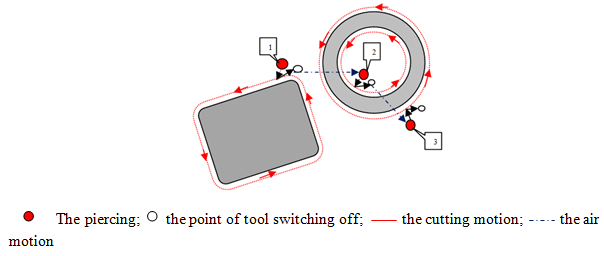
\includegraphics[width=0.9\textwidth]{elements.png}
  \caption{Cutting scheme example of two parts using standard cutting technique}
  \label{elements}
  \end{center}
\end{figure}

During development of NC program the optimization problems of cutting tool path are arisen.
The cutting cost $F_{cost}$ are one of numerical characteristics
that defines the effectiveness of NC program for special set of parts.
$F_{cost}$ is calculated by \cite{ru04}:

\begin{equation}
F_{cost} =
L_{on} \cdot C_{on} +
L_{off} \cdot C_{off} +
N_{pt} \cdot C_{pt}
\to \min
\label{cost}
\end{equation}

$L_{on}$ is length of air tool path;
$L_{off}$ is length of working tool path;
$C{on}$ is cost of air tool path unit;
$C_{off}$ is cost of working tool path unit;
$N_{pt}$ is numbers of piercing;
$C_{pt}$ is cost of one piercing.

In general when using different types ($j = \overline{1, k}$) of piercing
the $F_{cost}$ is calculated by:

\begin{equation}
  F_{cost} =
  L_{on} \cdot C_{on} +
  L_{off} \cdot C_{off} +
  \sum_{j=1}^k L_{pt}^j \cdot C_{pt}^j
  \to \min
  \label{cost-n}
\end{equation}

The problem of cost function minimization is considered as
\textit{generalized travelling salesman problem (GTSP) with restrictions}
\cite{ru04,ru05}.
The formalization of minimization problem of cutting time and cost
for CNC sheet cutting machines is presented in \cite{ru04}.

In \cite{Dewil2016Nov,Hoeft1997Sep}
the following classes of cutting tool routing problems
for CNC sheet cutting machines are allocated:

\begin{itemize}

\item The Traveling Salesman Problem – TSP;

\item The Generalized Traveling Salesman Problem – GTSP;

\item The Continuous Cutting Problem – CCP;

\item The End Point Cutting Problem – ECP;

\item Intermittent Cutting Problem – ICP;

\item Based on conception of contours cutting by segment \cite{Petunin2015Nov}
the new class of optimization tool routing problem is presented:
Segment Continious Cutting Problem (SCCP).

\end{itemize}

In optimization problem (\ref{cost-n})
there are difficulties in calculating the basic parameters
$C_{on}, C_{off}, C_{pt}$,
depending on many factors.
For CNC laser cutting machines $C_{on}, C_{off}, C_{pt}$
depend on the type of laser used in CNC machine,
type and thickness of treatment material.
The dependence on selected factors is defined by analytically or tabular functions.
The formulas of $C_{on}, C_{off}, C_{pt}$
calculation and their values may significantly differ for various CNC sheet cutting machines.
It is worth noting that time per pierce in laser cutting process is calculated in \cite{ru06}.
In \cite{ru07} the laser cutting cost is compared with water jet,
plasma and oxygen cutting costs when treatment sheet material of St3
(thicknesses $\Delta=3-10$ mm).
In \cite{ru08} the assessment of plasma and $CO_2$ laser cutting machines operating cost is performed.
But it should be noted that the calculation of mentioned above parameters
remains outside the scope of modern research,
hence the research for $C_{on}, C_{off}, C_{pt}$
calculation and consequently exact calculation of cost function $F_{cost}$
is actual problems today, which is solved in this article.

As seen from (\ref{cost-n})
$F_{cost}$
also depends on
$L_{on}, L_{off}$ and $N_{pt}$,
in turn $L_{on}$ depends on value of working tool speed $V_{on}$.
The value of $V_{on}$ is usually constant parameter
which is programming during the NC program development,
but as the practical shows \cite{ru09,Tavaeva2015Nov}
the value of actual working speed of cutting tool
is varied by various technological factors and parameters of NC programs.
Consequently problem of accurate calculation of cost function \ref{cost-n}
in optimization problem of tool path routing is arisen.
In order to solve the encountered problem
the need of correction parameters calculation for $V_{on}$
values is emerged.
It should be noted that
the question of exact calculation of  $V_{on}$ values remains open,
then there is a need of research in order to calculate the correction parameters of  $V_{on}$
values and consequently cutting cost in this article for CNC laser cutting machines.

It is observed that $L_{on}, L_{off}$ and $N_{pt}$
are interdependent.
In some cases the reduction of  $N_{pt}$
leads to some increase of total cutting tool path length value $L_{on}$
due to cutting motion between contours.
Wherein the length of air path $L_{off}$ is reduced.

The problem of cost function minimization (\ref{cost-n})
during treatment of figured parts from sheet material
at CNC cutting machines is solved by the optimization of parameters
$L_{on}, L_{off}$ and $N_{pt}$.
As the practice shows the length of cutting tool motion  $L_{on}$
and numbers of pierce points $N_{pt}$
have the greatest impact on the cutting cost compared with the length of air tool motion $L_{off}$.
Depending on the thickness and type of material the $C_{pt}$
can reach up to 33\% from $C_{on}$
and at the same time can exceed the $C_{off}$
by three orders \cite{ru14}.
Consequently the most interest are the methods of solving the problem aimed at the minimizing
$L_{on}$ and $N_{pt}$.

Analyze of existing methods of cost function minimizing showed that
airtime and length of air motion are usually minimized when optimizing the path of cutting tool.
In some works an algorithms for optimizing the airtime of cutting tool are considered.
Yang et al. \cite{Yang2010}
described the tool path airtime optimization problem in leather cutting.
They proposed the hybrid intelligence algorithm.
Castelino et al. \cite{d2003tool}
described an algorithm for minimizing the airtime of cutting tool
by optimally connecting the tool path.
They considered the heuristic methods that are used
in order to obtain the optimal or near optimal solutions.
Murzakaev et al \cite{ru17} considered the problem of cutter air motion length minimization.
The model is presented for standard cutting technique.
In order to minimize cutter air motion length the three metaheuristics
(Simulated Annealing, Threshold Accepting, Great Deluge Algorithm) were chosen.
They proposed the generalized scheme of problem solving.
Chen et al \cite{Chen2014Dec}
proposed algorithm of air motion path minimizing.
They divided into two sub-optimal problems
(pattern cutting order and entry/exit cutting point)
and solve ones using an ant colony optimization algorithm (min-max ant system).
Lee and Kwon \cite{Lee2006Dec}
considered tool path problem and proposed two-step genetic algorithm.
The aim is to minimize the air moving of cutting tool.
They combined global search for piercing optimization and local search for part sequencing.
Sherif et al \cite{Sherif2014Oct}
presented the two stage sequential optimization procedure for nesting and cutting sequence.
The objectives are maximizing material utilization and minimization of laser cutting tool air motion.
They considered simulated annealing algorithm in order to find the near optimal cutting tool path.

It should be noted that
the deficiency of research in the field of reducing the numbers of pierce points $N_{pt}$
and length of cutting tool motion  $L_{on}$
in solving the optimization problem (\ref{cost-n}).
In \cite{Manber1984Jan}
the authors consider the problem of pierce point numbers reducing
in thermal cutting of sheet material in terms of graph theory.
It should be noted that the precedence constrain was not taken into account
and the intersection of the existing cuts is allowed.
The problem of cutting path optimization in terms of cutting of parts group
with one of pierce point is considered in \cite{ru22}.
The last stage of solving the problem
(optimization of the cutter routing at idle)
is reduced to the TSP.
In \cite{ru23} the problem of tool routing optimization at CNC machines is formulated
and the mathematical model of total cutting time minimization is proposed
by using standard and special cutting techniques.
Verhoturov et al. \cite{ru24} present ``chained'' cutting technique
in order to minimize the numbers of pierce points.

The one of cutting time and cost minimization methods is
application of special cutting techniques.
In order to optimize the cutting parameters
and to observe the necessary cutting requirements
the some special cutting techniques are used.
There are ``chained'' cutting [24],
common cut \cite{ru25}, partial cutting of contour
with the subsequent completion of the contour cutting
after cutting the contour of another part, et al.
Petunin and Krotov \cite{ru25} proposed the
classification of various cutting techniques
used to form the cutting tool path.
The cutting techniques are classified into three main classes:
standard cutting, multi-contour cutting and multi-segment cutting technique.
The every contour is cut with pierce point by using
\textit{standard cutting technique}.
The numbers of pierce points equal numbers of contours.
The several contours are cut in one cutting segment
with one pierce point by using
\textit{multi-contour cutting technique}.
For example, the multi-contour cutting includes ``chained'' cutting, common cut.
The several cutting segments are cut with several pierce points by using
\textit{multi-segment technique}.

The considered techniques applied for various types of parts
and their effectiveness for different types are varied.
In some cases the effectiveness reaches the minimum value.
For this reason in order to minimize $F_{cost}$
the development of special cutting techniques
for various geometrical types of parts is actual problem today.
The circle, polygon parts are often found during sheet-working production
in engineering industry.
The treatment of parts without additional cut is impossible
with the help of the existing multi-contour cutting techniques.
Due to this fact the special cutting technique
for circle and polygon parts is proposed in this article.

The article is organized as follows.
The model of $F_{cost}$
calculation and basic parameters
$C_{on}, C_{off}, C_{pt}$
is presented in Section 2.1.
Exact calculation of $V_{on}$
values and values of correction coefficients for $V_{on}$
is given in Section 2.2.
The special cutting technique for circle and polygon parts
is proposed in Section 3.
The results of the computational experiment,
which shows a statistically significant improvement
in the value of the objective function
compared to using the standard cutting technique,
are presented in Section 4.

\section{Exact calculation of cost function $F_{cost}$ in cutting sheet material at CNC laser $CO_2$ machine}

\subsection{Model of basic cost parameters  $C_{on}, C_{off}, C_{pt}$ calculation}

The most important economic characteristic of the developed NC program quality is the cost $F_{cost}$
of cutting parts at CNC machine.
$F_{cost}$ includes the costs of electricity and expendable materials,
maintenance of a CNC machine and other operating costs incurred during cutting.
The problem of exact calculation of cost function $F_{cost}$
in optimizing of cutting tool route related with search of adequate value  $F_{cost}$,
which calculation depends on basic parameters  $C_{on}, C_{off}, C_{pt}$.

The problem of accurate calculation of cutting cost
in optimization problem of cutting tool routing applied to CNC laser cutting machine
(laser type is $CO_2$)
is considered.
In order to calculate $C_{on}$
the following notations for cost parameters calculation on 1 m of cutting tool motion are entered:
$C_{exp.mat}$ - the cost of expendable materials
(for example, adjudge, protective glass, gas tubes);
$C_{tech}$  - the cost of technological gas
(nitrogen or oxygen depending on processed material);
$C_{las}$ - the cost of cutting gas
(when working on a gas flow laser);
$C^{on}_{elec}$ - the cost of electricity;
$C^{on}_{salary}$ - the cost related with salary of accompanying personnel;
$C^{on}_A$ - amortization of equipment.
In general the  is calculated by:

\begin{equation}
C_{on} =
C^{on}_{elec} + C_{tech} + C_{las} + C_{exp.mat} + C^{on}_{salary} + C^{on}_A
\label{eq1.3}
\end{equation}

In order to calculate
$C^{on}_{elec}, C_{tech}, C_{las}, C_{exp.mat}, C^{on}_{salary}, C^{on}_A$
the additional notations are entered:
$t_{on}$  - the time spent on 1 m of cutting tool motion, h.;
$P_{on}$  - the electricity costs for 1 hour of CNC laser machine work on cutting motion, $kW/h$;
$V_{tech}$  - technological gas consumption, $m^3/h$ ;
$V_{las}$ - laser gas consumption, $m^3/h$;
$C_{elec}$  - electricity cost per 1 kW;
$C_{las M^3}$  - the cost of 1 $m^3$ laser gas;
$C_{tech M^3}$  - the cost of 1 $m^3$ technological gas;
$C_{exp.mat.Unit}$  - the cost of expendable materials unit;
$t_{exp.mat.Term}$  - serviceable life of expendable materials;
$C_{salary}$ - cost of 1 h work of accompanying personnel;
$A$ – amortization of 1 h work of CNC laser cutting machine;
$N$ - useful life of equipment;
$C_{equip}$  - initial cost of the CNC laser cutting machine.
They are thus calculated:

\begin{equation}
\label{eq1.4}
C^{on}_{elec} = P_{on} t_{on} C_{elec}
\end{equation}

\begin{equation}
  \label{eq1.5}
  C_{tech} = V_{tech} C_{tech M^3} t_{on}
\end{equation}

\begin{equation}
  \label{eq1.6}
  C_{las} = V_{las} C_{las M^3} t_{on}
\end{equation}

\begin{equation}
  \label{eq1.7}
  C_{exp.mat} = \frac{C_{exp.mat.Unit} t_{on}}{t_{exp.mat.Term}}
\end{equation}

\begin{equation}
  \label{eq1.8}
  C^{on}_{salary} = C_{salary} t_{on}
\end{equation}

\begin{equation}
  \label{eq1.9}
  C^{on}_A = \frac{1}N \frac{C_{equip}}{1920} t_{on}
\end{equation}

In order to calculate $C_{off}$
the following notations are entered:
$P_{off}$ – the electricity costs for 1 hour of CNC laser machine work on air motion, $kW/h$;
$t_{off}$ – the time spent on 1 m of air tool motion, h.

\begin{equation}
  \label{eq1.10}
  C_{off}
  = P_{off} t_{off} C_{elec}
  + C_{salary} t_{off}
  + \frac{1}N \frac{C_{equip}}{1920} t_{off}
\end{equation}

In order to calculate $C_{pt}$
the following notations for cost parameters calculation on 1 pierce point are entered:
$C^{pt}_{exp.mat}$ - the cost of expendable materials
(for example, adjudge, protective glass, gas tubes);
$C^{pt}_{tech}$ - the cost of technological gas
(nitrogen or oxygen depending on processed material);
$C^{pt}_{las}$ - the cost of cutting gas
(when working on a gas flow laser);
$C^{pt}_{elec}$ - the cost of electricity;
$C^{pt}_{salary}$ - the cost related with salary of accompanying personnel;
$C^{pt}_A$ - amortization of equipment.

\begin{equation}
  \label{eq1.11}
  C_{pt}
  = C^{pt}_{elec}
  + C^{pt}_{exp.mat}
  + C^{pt}_{las}
  + C^{pt}_{tech}
  + C^{pt}_{salary}
  + C^{pt}_A
\end{equation}

In order to calculate $C^{pt}_{elec}, C^{pt}_{exp.mat}, C^{pt}_{las}, C^{pt}_{tech},
C^{pt}_{salary}, C^{pt}_A$
the additional notations are entered:
$P_{pt}$ – the electricity costs for 1 pierce point, $kW/h$;
$t_{pt}$  – the time spent on 1 pierce point, h.

\begin{equation}
  \label{eq1.12}
  C^{pt}_{elec} = P_{pt} t_{pt} C_{elec}
\end{equation}

\begin{equation}
  \label{eq1.13}
  C^{pt}_{exp.mat} = V_{tech} C_{tech M^3} t_{pt}
\end{equation}

\begin{equation}
  \label{eq1.14}
  C^{pt}_{las} = V_{las} C_{las M^3} t_{pt}
\end{equation}

\begin{equation}
  \label{eq1.15}
  C^{pt}_{exp.mat} = \frac{C_{exp.mat.Unit} t_{pt}}{t_{exp.mat.Term}}
\end{equation}

\begin{equation}
  \label{eq1.16}
  C^{pt}_{salary} = C_{salary} t_{pt}
\end{equation}

\begin{equation}
  \label{eq1.17}
  C^{pt}_A = \frac{1}N \frac{C_{equip}}{1920} t_{pt}
\end{equation}

During calculation of $C_{pt}$
and $C_{on}$
the following parameters $C^{pt}_{las}$
and $C_{las}$ must be taken into account
when processing of material at flow-through gas laser machines.
The parameter $C^{pt}_{tech}$
must be considered during calculation of $F_{cost}$
when technological gas is applied.

Consequently, $F_{cost}$
can be written as follows:

\begin{multline}
  \label{eq1.18}
  F_{cost}
  = L_{on} \Big(
    C^{on}_{elec} + C_{tech} + C_{las} + C_{exp.mat} + C^{on}_{salary} + C^{on}_A
    \Big)
  + L_{off} C_{off} \\
  + N_{pt} \Big(
    C^{pt}_{elec} + C^{pt}_{exp.mat} + C^{pt}_{las} + C^{pt}_{tech} + C^{pt}_{salary} + C^{pt}_A
    \Big)
\end{multline}

The main expendable materials for gas laser include:
swivel mirrors, focusing lenses, protective glasses, nozzles, adjusting units, gas tubes.
The main expendable materials for fiber laser are nozzles, protective glasses, focusing lenses.
And for the case of using solid-state lasers,
the expendable materials are
optical pumping lamps, protective glasses, mirrors, a quantron, an active element.
In \cite{ru14} the values of cost parameters
$C_{on}, C_{off}, C_{pt}$
are presented by taken into account the above parameters (\ref{eq1.3})-(\ref{eq1.17})
for CNC laser cutting machine by example ByStar 3015.
For each type of material the parameters $C_{on}, C_{off}, C_{pt}$
are calculated by taken into account that
$V_{on}=const$.
As the practical shown \cite{ru09,Tavaeva2015Nov}
the value of actual working speed of cutting tool
is varied by various technological factors and parameters of NC programs.
Consequently problem of accurate calculation of cost function (\ref{cost-n})
in optimization problem of tool path construction is arisen.
In order to solve the encountered problem
the need of correction parameters calculation for $V_{on}$
values is emerged.

\subsection{Calculation of cutting tool speed $V_{on}$
and correction coefficient depending on the complexity of
part contours by example of the CNC laser cutting machine ByStar 3015}

The inaccuracy of the actual cutting time and cost calculation is due to the fact that $V_{on}$,
which is programmed as constant value in NC program,
is actually varied by various technological factors.
It was found that increasing of frames numbers in NC program
for various sets of parts,
which have the same total perimeter of the contours,
the actual $V_{on}$ is decreased \cite{ru09,Tavaeva2015Nov}.
The reasons why NC program can contain a large numbers of frames
is mainly due to the contours of complex geometry (for example, splines)
when converting from CAD systems to a CAM
are divided into a large numbers of geometric primitives
due to the difference of geometric file formats
(for example, on segments of straight lines and circular arcs),
i.e. approximated by simple geometric primitives.
The difference in formats is due to the fact that
almost all CNC systems are equipped with only linear and circular interpolators.
As a rule the approximation of a complex geometry reduces to a linear approximation.

The functional dependence of $V_{on}$
should be determined by science-based table functions or analytically.
The algorithmization of objective function (\ref{cost-n})
calculation based on science–based determination of function parameters
is requirement for the development of cutting tool path optimization algorithms.
The cutting tool route is optimal only if
the objective function is adequate calculated.
For this reason the exact parameters values of objective function (\ref{cost-n})
must be calculated.

The some practical results on determining
the dependence of cutting tool speed on numbers of frames in NC program
are given below [10].
Based on received results the objective function (\ref{cost-n})
can exactly calculated and optimal cutting tool route can developed.

The research was conducted for following materials:
1.4541 (thickness $\Delta=1-10$ mm) and
AWAIMg3 (thickness $\Delta=1-10$ mm).
In order to conduct experiments the 150 NC programs
for cutting of various types of parts with numbers of frames
$n=\overline{4, 5092}(n \in \mathbb{N})$
for 1.4541
and 150 NC programs for cutting of various types of parts with numbers of frames
$n = \overline{10, 1962} (n \in \mathbb N)$
for AWAIMg3.

The statistical materials were processed by using ``Mathcad''.
Based on received results the following findings were made:

\begin{enumerate}
\item
The actual average speed of cutting tool speed $V_{act}$
is monotonically decreasing function depending on frames numbers of NC program
(Fig. \ref{plot});

\item
The predetermined cutting tool speed $V_{on}$
coincides with the actual average speed
when the numbers of frames reaches a certain threshold value $N$.
When the frames numbers $n < N$,
then the actual speed is greater than predetermined cutting tool speed,
if the frames numbers of NC program is arisen ($n>N$)
then the actual speed is less than
predetermined cutting tool speed of NC program
(in the experiments the reduction of average actual cutting tool speed value
compared with predetermined cutting tool speed in NC program is 70\%);

\item
The threshold value $N$ is varied for different thickness and grade of material.
\end{enumerate}

\begin{figure}
  \begin{center}
  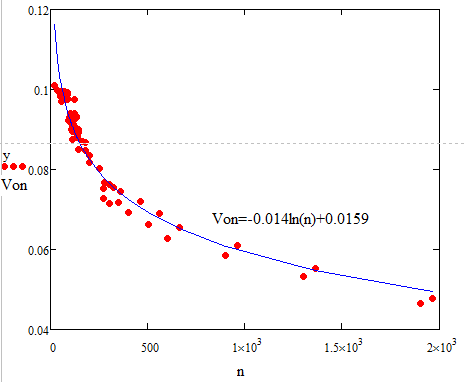
\includegraphics[width=0.8\textwidth]{plot.png}
  \caption{Change of the real cutting tool speed for AWAIMg3, $\Delta=1$ mm}
  \label{plot}
  \end{center}
\end{figure}

In order to present the results of computational experiments
the following notations are introduced:
$n$ – frames numbers of NC program;
$V_{act}$ - the actual speed of cutting too;
$N$ – the frames numbers when $V_{act}=V_{on}$;
$\sum_n e_n^2$  - the sum of squared deviations of the
original data from the values of the approximation functions at these points.

When approximation the point chart
of the dependence of actual speed
on the numbers of frames by approximating curves in ``Mathcad''
it was established for all values of studied grade materials
and thickness that values of $\sum_n e_n^2$
are achieved by using logarithmic approximation function.
Fig. \ref{plot} presents following results for material of AWAIMg3 with $\Delta=1$ mm.

Similar results were obtained for AWAIMg3 with $\Delta=2-5$ mm
and 1.4541 with $\Delta=1-10$ mm.
The generalized formulas for calculating of cutting tool speed
by example CNC laser cutting machine ByStar3015 are presented in \cite{ru28}.

\section{Special cutting techniques used during optimization of cutting tool route}

The one method of cutting time and cost minimization is application of special cutting techniques.

In engineering industry the geometrical forms of most parts are polygon and circle.
This paper considers the special cutting techniques for polygons and circles parts.
The special cutting techniques use more complexity algorithm in contrast to standard cutting technique.

In \cite{ru26} the cutting techniques for circle and triangle parts were proposed.
The effectiveness conditions of proposed techniques were obtained.
Solving problem of irregular cutting the method of parts association
in group or ``block'' is often used.
During nesting the ``block'' is similarly the one part,
i.e. the all movements / rotations are made simultaneously
with all the details included in the ``block''.
The association in ``blocks'' is actually in our case.
Fig. \ref{8} presents the scheme of circle parts cutting using special cutting technique.

The continuous cutting of parts is performed.
At first the upper sectors are cut.
At second the lower sectors are cut last.
Wherein moving from one sector to another is implemented by cutting motion (Fig. \ref{8}).
The proposed cutting technique reduces the number of piercing, air motions,
but increases the cutting motion.
Consequently the cutting motion length of cutter needs to be taken into account
when moving from one contour to another.
These cutting costs should not exceed the costs of piercing.
Based on results \cite{ru26},
the algorithm of cutting tool route automation for CAD/CAM ``SIRIUS'' was developed.
While cutting tool routing the Part Hardness Rule is taken into account \cite{ru27}.
The proposed algorithm is applicable for any size circles
and allows to automatically build the cutting tool route.

\begin{figure}
  \begin{center}
  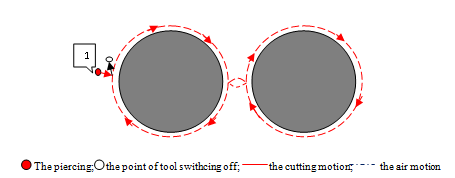
\includegraphics[width=0.9\textwidth]{8.png}
  \caption{Cutting scheme example of two parts using special cutting}
  \label{8}
  \end{center}
\end{figure}

The special cutting technique for triangle parts was proposed \cite{ru26}.
In engineering manufacturing the most geometrical form of parts is polygon.
Therefore the algorithm of cutting tool route automation for polygon parts
was developed based on proposed special cutting technique for CAD/CAM ``SIRIUS''.
While cutting tool routing the Part Hardness Rule is taken into account \cite{ru27}.
The algorithm can be used by designing NC program in interactive mode.
The features of proposed technique are the reducing of piercing,
the cutting and air motions of cutter.
The proposed algorithm is applicable for various one-sided symmetry polygons.
The proposed technique significantly reduces numbers of piercing,
cutting and air motions of cutter for polygon parts.
The polygons can be arranged in the cell type.
Fig. \ref{tri} presents the cutting scheme of triangle parts.
The parts are combined by ``blocks'' and within each ``block''
the cutting is performed by one piercing.
Moving from one ``block'' to another is implemented by air.

\begin{figure}
  \begin{center}
  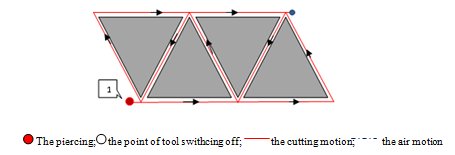
\includegraphics[width=0.9\textwidth]{tri.png}
  \caption{Cutting scheme example of four triangle parts using special cutting techniques}
  \label{tri}
  \end{center}
\end{figure}

In order to evaluate the effectiveness
of developed special cutting techniques
the computing experiments were conducted at CAD/CAM ``SIRIUS''
and obtained results is presented in Section 4.

\section{Computational experiments}

Based on algorithms presented on Section 3
the cutting tool route for nesting is automatically built at CAD/CAM ``SIRIUS''.
In order to evaluate the the effectiveness of developed special cutting techniques
the four nesting is obtained by using standard (Fig. \ref{cut-std}, \ref{poly-std})
and special (Fig. \ref{cut-spec}, \ref{poly-spec})
cutting techniques for various types of parts including circles
(Fig. \ref{cutting}) and polygon (Fig. \ref{polygons}) parts.

Fig. \ref{cut-std} presents the cutting tool path
built for various geometrical types of parts including circles using standard cutting techniques.
Fig. \ref{cut-spec} presents the cutting tool path built for various geometrical types of parts
including circles using special cutting techniques.

\begin{figure}
  \centering
  \subfigure[Standard cutting technique]{
    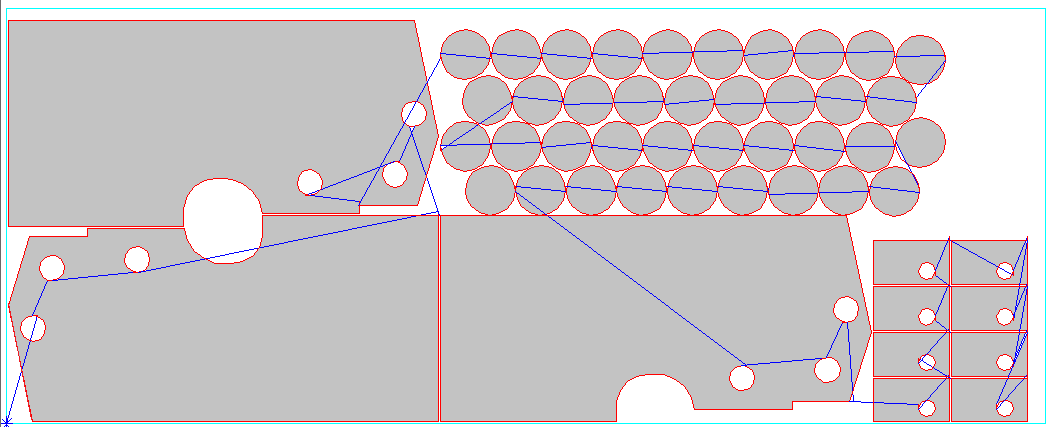
\includegraphics[width=0.47\textwidth]{std.png}
    \label{cut-std}
  }
  \subfigure[Special cutting technique]{
    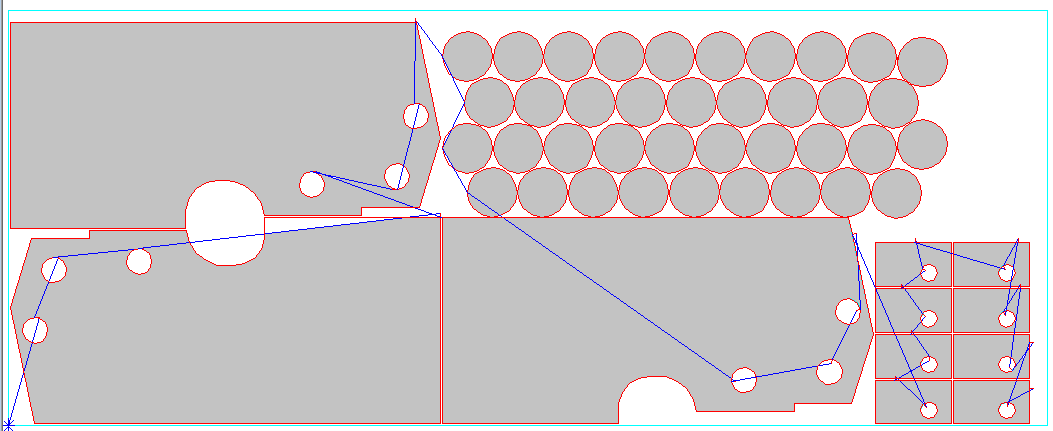
\includegraphics[width=0.47\textwidth]{special.png}
    \label{cut-spec}
  }
  \caption{Cutting scheme example}
  \label{cutting}
\end{figure}

Table \ref{f-cost} presents computational results of basic cutting parameters and values of $F_{cost}$
for obtained NC programs developed based on cutting tool path for nesting
(Fig. \ref{cutting}, \ref{polygons}).
The calculation of $F_{cost}$
was carried out by using model presented in Section 2.1 and 2.2.
The results are calculated for AWAIMg3 $\Delta = 5$ mm.
The following notations in table 2 are used:
$n$ – numbers of frames in NC program;
$F_{cost}$ - the cutting cost calculated taking into account that $V_{on}=const$;
$F^n_{cost}$ - the cutting cost calculated taking into account that $V_{on}=var$  and depends on the frames numbers of NC program.

Fig. \ref{poly-std}
presents the cutting tool path built for various geometrical types of parts
including polygons and circles using standard cutting techniques.
Fig. \ref{poly-spec} presents the cutting tool path built for various geometrical types of parts
including polygons and circles using special cutting techniques.

\begin{figure}
  \centering
  \subfigure[Standard cutting technique]{
    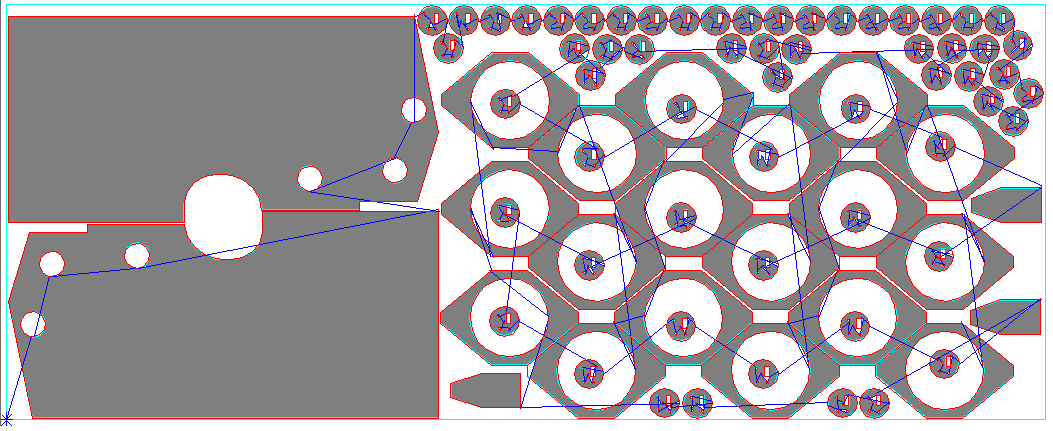
\includegraphics[width=0.47\textwidth]{spec-a.png}
    \label{poly-std}
  }
  \subfigure[Special cutting technique]{
    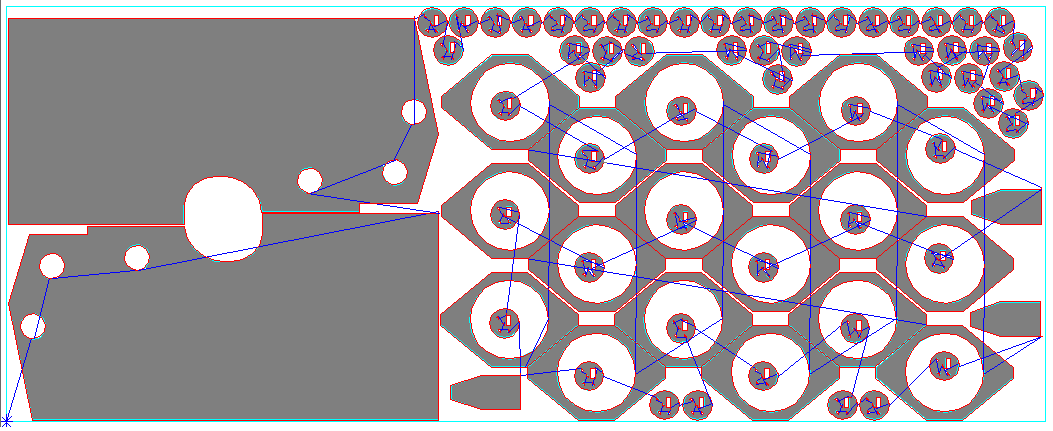
\includegraphics[width=0.47\textwidth]{spec-b.png}
    \label{poly-spec}
  }
  \caption{Cutting scheme example of special part shapes}
  \label{polygons}
\end{figure}

The results presented in Table \ref{f-cost} indicate that
the basis cutting parameters are reduced by using special cutting techniques
compared with standard cutting.
In turn the reduction of $N_{pt}$, $L_{on}$ and $L_{off}$
leads to reduction of $F_{cost}$ by 4-5\%
using special cutting technique
compared with standard cutting.

\begin{table}
  \begin{tabular}{c | c | c | c | r r r | c | r r | r}
  Material & $\Delta$ & Technique & Fig. & $N_{pt}$ & $L_{on}, m$ & $L_{off}, m$ & $n$ & $F_{cost}$ & $F^n_{cost}$ & \% \\
  \hline \hline
  \multirow{4}{*}{AWAIMg3} & \multirow{4}{*}{5 mm} & Standard & Fig. \ref{cut-std}     & 66  & 63.3   & 20.34 & \multirow{2}{*}{169} & 22908.32 & 28519.79 & \multirow{2}{*}{4.5} \\
                         &                    & Special  & Fig. \ref{cut-spec} & 32  & 63.55  & 11.46 &                      & 21890.75 & 27524.38 & \\
                         &                    & Standard & Fig. \ref{poly-std}  & 407 & 117.78 & 50.47 & \multirow{2}{*}{888} & 51790.31 & 67100.44 & \multirow{2}{*}{4.7}\\
                         &                    & Special  & Fig. \ref{poly-spec}  & 361 & 114.93 & 47.61 &                      & 49371.17 & 64310.82 & \\
  \hline
  \end{tabular}
  \caption{Results of $F_{cost}$ calculation}
  \label{f-cost}
\end{table}

\section{Conclusion}

In this article the following results were obtained:

\begin{enumerate}

\item  The problem of cutting tool path optimization on CNC machines was considered.
The model of cost function $F_{cost}$ and basic parameters calculation is presented for CNC laser cutting machines.
$F_{cost}$ includes the costs of electricity and expendable materials,
maintenance of a CNC machine and other operating costs incurred during cutting.
The problem of exact calculation of cost function  $F_{cost}$
in optimizing of cutting tool route related with search of adequate value  $F_{cost}$,
which calculation depends on basic parameters $C_{on}, C_{off}, C_{pt}$

\item The value of actual working speed of cutting tool is varied
by various technological factors and parameters of NC programs.
The problem of accurate calculation of cost function (1.2)
in optimization problem of tool path construction is solved in this article.
The correction parameters for $V_{on}$ values
is presented for type of material AWAIMg3 ($\Delta=1-5$ mm) and St1.4541 ($\Delta=1-10$ mm)

\item The one of cutting time and cost minimization methods is application of special cutting techniques.
In order to optimize the cutting parameters and to observe the necessary cutting requirements
the some special cutting techniques are used.
In this article the effective special cutting techniques
for the common geometrical types of parts
widely used in blank production of engineering plant are developed

\item The computational experiments shown that
application of presented special cutting technique allows to
reduce the basic cutting parameters of $N_{pt}, L_{on}$
and $L_{off}$ compared with standard cutting techniques.
The calculation of $F_{cost}$ is performed by model presented in Section 2.1.
In turn the calculation of  $F_{cost}$ is carried out by values of
$V_{on}=const$ and $V_{on}=var$
the results show value of $F_{cost}$ when $V_{on}=const$  is 30\% lower
than value of $F_{cost}$  when $V_{on}=var$.
The basic parameters of $N_{pt}, L_{on}$
and $L_{off}$
are reduced.
For example, when using the special cutting technique
$N_{pt}$ is reduced by 11\%  compared with standard cutting.
The reduction $N_{pt}, L_{on}$
and $L_{off}$
leads to reduction of $F_{cost}$ by 4-5\%
using special cutting technique (Fig. \ref{cut-spec}, \ref{poly-spec})
compared with standard cutting (Fig. \ref{cut-std}, \ref{poly-std}).

\end{enumerate}

\bibliographystyle{splncs04}
\bibliography{tavaeva}
\nocite{*}

\end{document}
